% Dokumenttyp
\documentclass[a4paper,11pt,twoside,german]{article}

% Befehle für Seitenränder
\newcommand{\largeborder}{3cm}
\newcommand{\smallborder}{2cm}
\newcommand{\topborder}{1cm}
\newcommand{\bottomborder}{1cm}

\usepackage[
    left=\largeborder,
    right=\largeborder,
    top=\topborder,
    bottom=\bottomborder,
    includeheadfoot,
    ]{geometry}
    
% \textwidth 16cm
% \textheight 24cm
%  \topmargin -15mm
% \setlength{\oddsidemargin}{-5mm}
% \setlength{\evensidemargin}{5mm}


%%%%%%%%%%%%%%%%%%%%%%%%%%
%%% Benötigte Packages %%%
%%%%%%%%%%%%%%%%%%%%%%%%%%

%%% Sprache %%%
\usepackage[ngerman]{babel}    	% damit man deutsche Dinge tun kann
\usepackage{ziffer} % Deutsche Zahlen

\usepackage[utf8]{inputenc}   % damit Umlaute funktionieren
\usepackage[autostyle=true,german=quotes]{csquotes} % Anführungszeichen richtig
\usepackage{blindtext} % damit man sinnlosen Text produzieren kann

%%% Grafiken %%%
\usepackage{graphicx}    % damit man Bilder einbinden kann
% \usepackage{float}    	% damit Floats da sind, wo sie hingehören
\usepackage{floatrow}   % bessere float Organisation
\usepackage[font=footnotesize,labelfont=bf,skip=0pt]{caption} %Captions anpassen
\addtolength{\intextsep}{2mm} % mehr Platz um figures und tables
\usepackage{subcaption}
\usepackage{pbox}


\usepackage{amsmath}  % damit abgefahrene mathematische Dinge in equations gehen
\usepackage{enumitem} % Damit Aufzählungen hübscher sind
\usepackage{ifthen}   % Damit man if-else-Strukturen machen kann

\setlength{\parindent}{0pt} % Keine Absatzeinrückung
\usepackage{setspace} % Zeilenabstände machen können
\linespread{1.05} % Zeilenabstand definieren
% Standardmäßig \absatz zur Trennung von Absätzen verwendet und hier anpassen
\newcommand{\absatz}{\smallbreak} 
%\renewcommand{\familydefault}{\sfdefault} % Serifenlose Schrift

%%% Links und Verweise %%%
\usepackage[breaklinks]{hyperref} % Damit Links funktionieren
\hypersetup{colorlinks=false,pdfborder={0 0 0}} % entferne hässliche Link-Kästen


%%% Bibliographie %%%
\usepackage[authoryear,round]{natbib} % Der Stil der LiteraturVERWEISE im Text
\bibliographystyle{dcu-german-spec} % Der Stil des LiteraturVERZEICHNISSES
%\bibliographystyle{dcu} % Der Stil des LiteraturVERZEICHNISSES


% Makro für Bibliographie
\newcommand{\literaturverzeichnis}[1]{
    \renewcommand{\harvardand}{und} % ein UND statt AND bei mehreren Autoren
    \bibliography{#1}
    }

% Literaturverzeichnis im Inhaltsverzeichnis, aber NICHT nummeriert
\usepackage[nottoc,notlot,notlof]{tocbibind} 
% Literaturverzeichnis nummeriert und im Inhaltsverzeichnis
% \usepackage[nottoc,numbib]{tocbibind}


% Commands to place things on a left or right side
% Put this before something you want to place either right 
% (onto the NEXT EVEN page) or left (onto the NEXT ODD page)
\newcommand{\emptypage}{\newpage\leavevmode\thispagestyle{empty}\newpage}
\newcommand{\fillwithemptypagestillevenside}{\ifthenelse{\isodd{\thepage}}
    {\emptypage}{}}
\newcommand{\fillwithemptypagestilloddside}{\ifthenelse{\isodd{\thepage}}{}
    {\emptypage}}

\newcommand{\breaktoevenside}{\ifthenelse{\isodd{\thepage}}{\newpage}{}}
\newcommand{\breaktooddside}{\ifthenelse{\isodd{\thepage}}{}{\newpage}}

% Metadaten
\usepackage{titling}
\title{LEX extended abstract}
\author{
    Büchau, Yann Georg \\
    \small{\texttt{64\,36\,211}}
    \and
    Finn, Tobias Sebastian \\
    \small{\texttt{00\,00\,000}}
    \and 
    Schaper, Maximilian \\
    \small{\texttt{64\,17\,160}}
    }
%%%%%%%%%%%%%%%%%%%%%%%%%%%%%%%%%%%%%%%%%%
\begin{document}
\raggedbottom


%%%%%%%%%%%%%%%%%%
%%% Titelseite %%%
%%%%%%%%%%%%%%%%%%

\hypersetup{pageanchor=false}
\makeatletter
\begin{titlepage}

%\newgeometry{
%    left=\smallborder,
%    right=\smallborder,
%    top=\topborder,
%    bottom=\bottomborder,
%    includeheadfoot,
%    }


\vspace*{\fill}
\begin{center}
\Large{\textbf{Lehrexkursion Fehmarn}}\\
\large{29.08.2016 - 09.09.2016}\\
\vspace{5mm}
\Large{\textbf{Arbeitsgruppe\\Stereo-Wolkenkamera}}\\
\vspace{1cm}

% authors
\begin{large}
\begin{tabular}{ccc}
Büchau, Yann Georg & Finn, Tobias Sebastian & Schaper, Maximilian \\
\small{\texttt{64\,36\,211}} & 
\small{\texttt{64\,80\,121}} &
\small{\texttt{64\,17\,160}}
\end{tabular}
\end{large}

\vspace{1cm}
\large{Meteorologisches Institut}\\
\large{Universität Hamburg}\\
\vspace{1cm}
\large{{\today}}
\end{center}
\vspace*{\fill}

\clearpage
% \restoregeometry


\end{titlepage}
\makeatother
\hypersetup{pageanchor=true}

\newpage

%%%%%%%%%%%%%%%%%%%%%%%%%%
%%% Inhaltsverzeichnis %%%
%%%%%%%%%%%%%%%%%%%%%%%%%%
\clearpage
\setcounter{page}{1} % Page counting begins here!

\tableofcontents % Inhaltsverzeichnis
\vspace*{\fill}

%%%%%%%%%%%%%%%%%%%%%%%%%%%%%
%%% Abbildungsverzeichnis %%%
%%%%%%%%%%%%%%%%%%%%%%%%%%%%%
%\listoftables % Abbildungsverzeichnis

\listoffigures % Abbildungsverzeichnis

\newpage


%%%%%%%%%%%%%%%%%%
%%% Motivation %%%
%%%%%%%%%%%%%%%%%%
\section{Einleitung}
Die Wolkenbasishöhe ist eine wichtige Größe in der Charakterisierung von Wolken,
da sie unter anderem maßgeblichen Einfluss auf ihre langwellige Ausstrahlung
hat.  Das klassische Gerät zur Ermittlung der Wolkenbasishöhe ist das
Ceilometer, welches Rückstreuprofile senkrechter Laser-Punktmessungen zur
Höhenbestimmung verwendet.  Auch Kameras haben als weiteres Instrument zur
Wolkenanalyse Verwendung gefunden. Anwendungsbereiche solcher Wolkenkameras
beinhalten die Bestimmung des Bedeckungsgrads, der Wolkenzuggeschwindigkeit und
-richtung sowie die Nowcast-Vorhersage für Solarkraftanlagen.\absatz Für viele
dieser Anwendungsbereiche bedarf es jedoch zumeist eines zusätzlichen
Ceilometers. Da diese allerdings recht kostspielig in der Anschaffung sind,
lohnt sich die Entwicklung alternativer Techniken der
Wolkenbasishöhenbestimmung. Eine solche Methode auf Basis eines
Stereo-Wolkenkamera-Aufbaus soll hier untersucht werden.  Dabei soll analog zum
klassischen Theodoliten-Doppelanschnitt mit zwei Wolkenkameras die Wolkenhöhe
trianguliert werden.\absatz Damit Wolkenpositionen im dreidimensionalen Raum
ermittelt werden können, sind mehrere Schritte notwendig: Kalibration der
Kameras (Kapitel\;\ref{SECCalib}), Wolkenerkennung
(Kapitel\;\ref{SECWolkenErkennung}) und Positionsbestimmung
(Kapitel\;\ref{SECHoehenbestimmung}). Eine Validierung erfolgt in
Kapitel\;\ref{SECValidation}.


%%%%%%%%%%%%%%
%%% Geräte %%%
%%%%%%%%%%%%%%
\section{Geräte}
\label{SECGeraete}

Die verwendeten zwei Kameras (Abb.~\ref{FIGKameras}) werden im Folgenden
\enquote{Acker} und \enquote{Feld} genannt. Es handelt sich um
Überwachungskameras VIVOTEK FE8174V mit einem Blickfeld von nahezu $180^\circ$
und einer Bildauflösung von $1920\,\mathrm{px} \cdot 1920
\,\mathrm{px}$.
\absatz

\begin{figure}[!h]
\begin{center}
\scriptsize
\begin{minipage}{0.45\textwidth}
    \bgroup
    \def\arraystretch{0.2}
    \begin{tabular}{cc}
    Kamera \enquote{\textbf{Acker}} & Kamera \enquote{\textbf{Zaun}} \\
    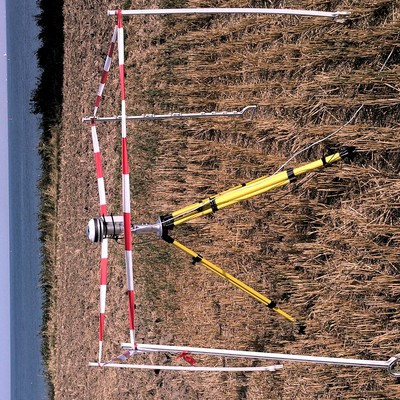
\includegraphics[width=0.45\textwidth, angle=-90]{media/cam4.jpg} &
    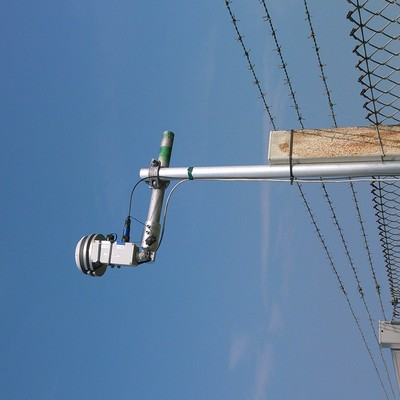
\includegraphics[width=0.45\textwidth, angle=-90]{media/cam3.jpg} \\
    \end{tabular}
    \egroup
\end{minipage}
\begin{minipage}{0.45\textwidth}
    \bgroup
    \def\arraystretch{2}
    \scriptsize
    \begin{tabular}{ccc}
    & 
    \pbox{\textwidth}{Kamera\\ \enquote{\textbf{Acker}}} &
    \pbox{\textwidth}{Kamera\\ \enquote{\textbf{Zaun}}} \\
    \hline
    \pbox{\textwidth}{\textbf{GPS Position}} & 
    \pbox{\textwidth}{$54,4959^\circ\,\mathrm{N}$ \\
    $11,2377^\circ\,\mathrm{O}$} &
    \pbox{\textwidth}{$54,4947^\circ\,\mathrm{N}$ \\ $11,2408^\circ\,\mathrm{O}$} \\
    \hline
    \pbox{\textwidth}{\textbf{Höhe über N.N.}} & 
    $0\,\mathrm{m}$ &
    $9\,\mathrm{m}$ \\
    \hline
    \end{tabular}
    \egroup
\end{minipage}
\vspace{-0.5cm}
\caption[Verwendete Kameras]{Kameras \enquote{Acker} und \enquote{Zaun} mit
Koordinaten. Kamera \enquote{Zaun} befand sich auf dem Militärgelände
Marienleuchte, Kamera \enquote{Acker} etwa $241\,\mathrm{m}$ entfernt auf einem
Feld.}
\label{FIGKameras}
\end{center}
\end{figure}


%\newpage % Neue Seite 

%%%%%%%%%%%%%%%%%%%
%%% Kalibration %%%
%%%%%%%%%%%%%%%%%%%
\section{Kalibration}
\label{SECCalib}
Grundlegend für die im Folgenden angewendete Triangulationsmethode ist die
Kenntnis des Azimuth- und Elevationswinkels in jedem Bildpunkt. Dazu ist eine
Kalibration der verwendeten Kameras erforderlich, mit der sowohl die radiale
Projektion der Kameralinse als auch die Drehungseffekte durch ungenaues
Aufstellen der Kamera quantifiziert werden können. Für eine derartige
Kalibration sind Raumpunkte nötig, deren Positionen sowohl auf dem Bild als auch
in der Realität bekannt sind. Es bietet sich hierfür die Sonne an, deren realer
Azimuth- und Elevationswinkel zu jedem Zeitpunkt berechenbar sind
\citep{pysolar}.
\absatz 
Wird die Kamera an einem nahezu wolkenlosen Tag mit Goldfolie bedeckt und die
Belichtungszeit verringert \citep{ingo}, erscheint die Sonne als einziger heller
Fleck auf dem ansonsten dunklen Bild (Abb.~ \ref{FIGFolie}). Das ermöglicht die
automatische Bestimmung der Sonnenposition auf dem Bild mittels Weichzeichnung,
Erosion kleiner Elemente und Mittelpunktsbestimmung des hellsten Bildbereichs.
\absatz Zur Bestimmung von Azimuth- und Elevationswinkel in jedem Bildpunkt wird
eine Projektion benötigt, mit der sich Bildkoordinaten $\left[Zeile \,\,
Spalte\right]$ in das reale, dreidimensionale Koordinatensystem
$\left[X\,\,Y\,\,Z\right]$ umrechnen lassen.  Eine solche Projektion ist in
Abbildung~\ref{FIGProjektion} gezeigt. Dabei wird zunächst anhand des Bildradius
$R_\mathrm{h}$, also des Abstandes des betrachteten Bildpunktes zur Bildmitte in
Bildpunktbreiten, der Lotwinkel $\phi$ zur optischen Achse angenährt. Er lässt
sich umrechnen in die Elevation $\epsilon = \frac{\pi}{2} - \phi$. Dem liegt die
Annahme zugrunde, dass es sich um eine radiale Verzerrung handelt, die
rotationssymmetrisch zur in der Bildmitte liegenden optischen Achse der Linse
ist.  Dieser Schritt quantifiziert also den Verzerrungseffekt der Linse. Hier
wird nach \cite{ingo} ein Polynom vierten Grades als Zusammenhang angenommen und
invertiert:

\begin{equation}
\label{GLRadial}
R_\mathrm{h} = p_4 \phi ^ 4 + p_3 \phi ^ 3 + p_2 \phi ^ 2 + p_1 \phi
\end{equation}

Durch die nun bekannte Elevation wird der Vektor des betrachteten Bildpunktes
dreidimensional. Zur Nordung wird der Vektor anschließend um den Winkel $\Phi_Z$
um die $Z$-Achse gedreht. Eine weitere Drehung um den Winkel $\Phi_X$ um die
$X$-Achse und um den Winkel $\theta_Z$ um die dann mitbewegte $Z$-Achse
korrigieren den Vektor um Fehler, die bei der Ze\-nit\-aus\-rich\-tung der
Kamera gemacht wurden. Diese drei Winkel $\Phi_Z$, $\Phi_X$ und $\theta_Z$
werden auch als Euler-Winkel bezeichnet.
\absatz
Die Kalibration kann als Optimierungsproblem betrachtet werden. Dazu
werden alle auf den Kamerabildern gefundenen Sonnenpositionen auf eine
Einheitssphäre im realen Koordinatensystem projiziert. Der mittlere quadratische
Abstand zu den tatsächlichen Sonnenpositionen auf der Einheitssphäre ist die zu
optimierende Kostenfunktion in Ab\-häng\-ig\-keit der Projetionsparameter $p_1$,
$p_2$, $p_3$, $p_4$, $\Phi_Z$, $\Phi_X$ und $\theta_Z$.
\absatz
Dieser Kalibrationsansatz lässt sich theoretisch sowohl für jede Aufstellung
einer Kamera, als auch für jede Art von Kamera anwenden. Allerdings wird es bei
anderen Kameras eventuell nötig sein, die radiale Projektionsfunktion in
Gleichung \ref{GLRadial} anzupassen, wenn sich die Art der Linse stark von der
hier verbauten unterscheidet.
\absatz
Die radiale Projektionsfunktion ist gerätespezifisch. Somit sind die Parameter 
$p_1$, $p_2$, $p_3$ und $p_4$ unabhängig von der Aufstellung. Daher bietet es
sich an, die Projektionsfunktion separat zu bestimmen und für jede
Kameraaufstellung zu übernehmen. Für eine optimale Genauigkeit sind
möglichst viele Sonnenpositionen auch in der Bildmitte erforderlich, was bei
einer Ausrichtung in den Zenit in den mittleren Breiten nicht erfüllt ist.
Wird die Kamera in Richtung der Mittagssonne ausgerichtet, ist diese
Vorraussetzung erfüllt, wie in Abb.~\ref{FIGFolie}(b) zu sehen ist.
Mit dieser Aufstellung ergeben sich für die Kamera \enquote{Zaun} 
die folgenden Radialprojektionsparameter:

\begin{equation}
p_4 = -20,933 \;\;\;\;
p_3 = 0,536   \;\;\;\;
p_2 = 25,295  \;\;\;\;
p_1 = 658,265 \;\;\;\;
\end{equation}

Da die beiden hier verwendeten Kameras baugleich sind, wird für Kamera
\enquote{Acker} dieselbe Projektionsfunktion angenommen.  Mit dieser
Projektionsfunktion (Abb.~\ref{FIGProjektioncalib}) können die in den
Zenit gerichteten Kameraaufstellungen kalibriert werden, wie etwa in Abbildung
\ref{FIGFolie}(a) zu sehen ist. Aus den daraus gewonnenen Parametern lassen sich für jeden Bildpunkt ein Azimuth- und Elevationswinkel bestimmen. 
\absatz 
Eine Koordinatentransformation kann dann dazu verwendet werden, die
Bilder zu entzerren. Dazu wird ein Gitter aus equidistanten $X$ und $Y$
Koordinaten erstellt und eine virtuelle, konstante Höhe $Z$ angenommen. Diese
virtuelle Höhe $Z$ hat keine Verbindung zu der Wolkenhöhe, sondern dient nur der
Darstellung einer Ebene. Aus diesen Koordinaten werden Azimuth und Elevation
berechnet und dann darauf das Kamerabild auf Basis seiner kalibrierten Azimuth-
und Elevationswinkel intepoliert.
Im Folgenden wird mit entzerrten Wolkenkamerabildern gearbeitet.

\begin{figure}[!h]
\begin{center}
\begin{floatrow}
\ffigbox{
    \caption[Sonnenbahn auf mit Goldfolie bedeckter Kamera]{
    Zusammenstellung ausgewählter Aufnahmen der mit Goldfolie bedeckten Kamera
    \enquote{Zaun} bei einer groben Ausrichtung der optischen Achse (Bildmitte)
    (a) in den Zenit und (b) in die Mittagssonne.
    }
    \label{FIGFolie}
}{
    \begin{tabular}{cc}
        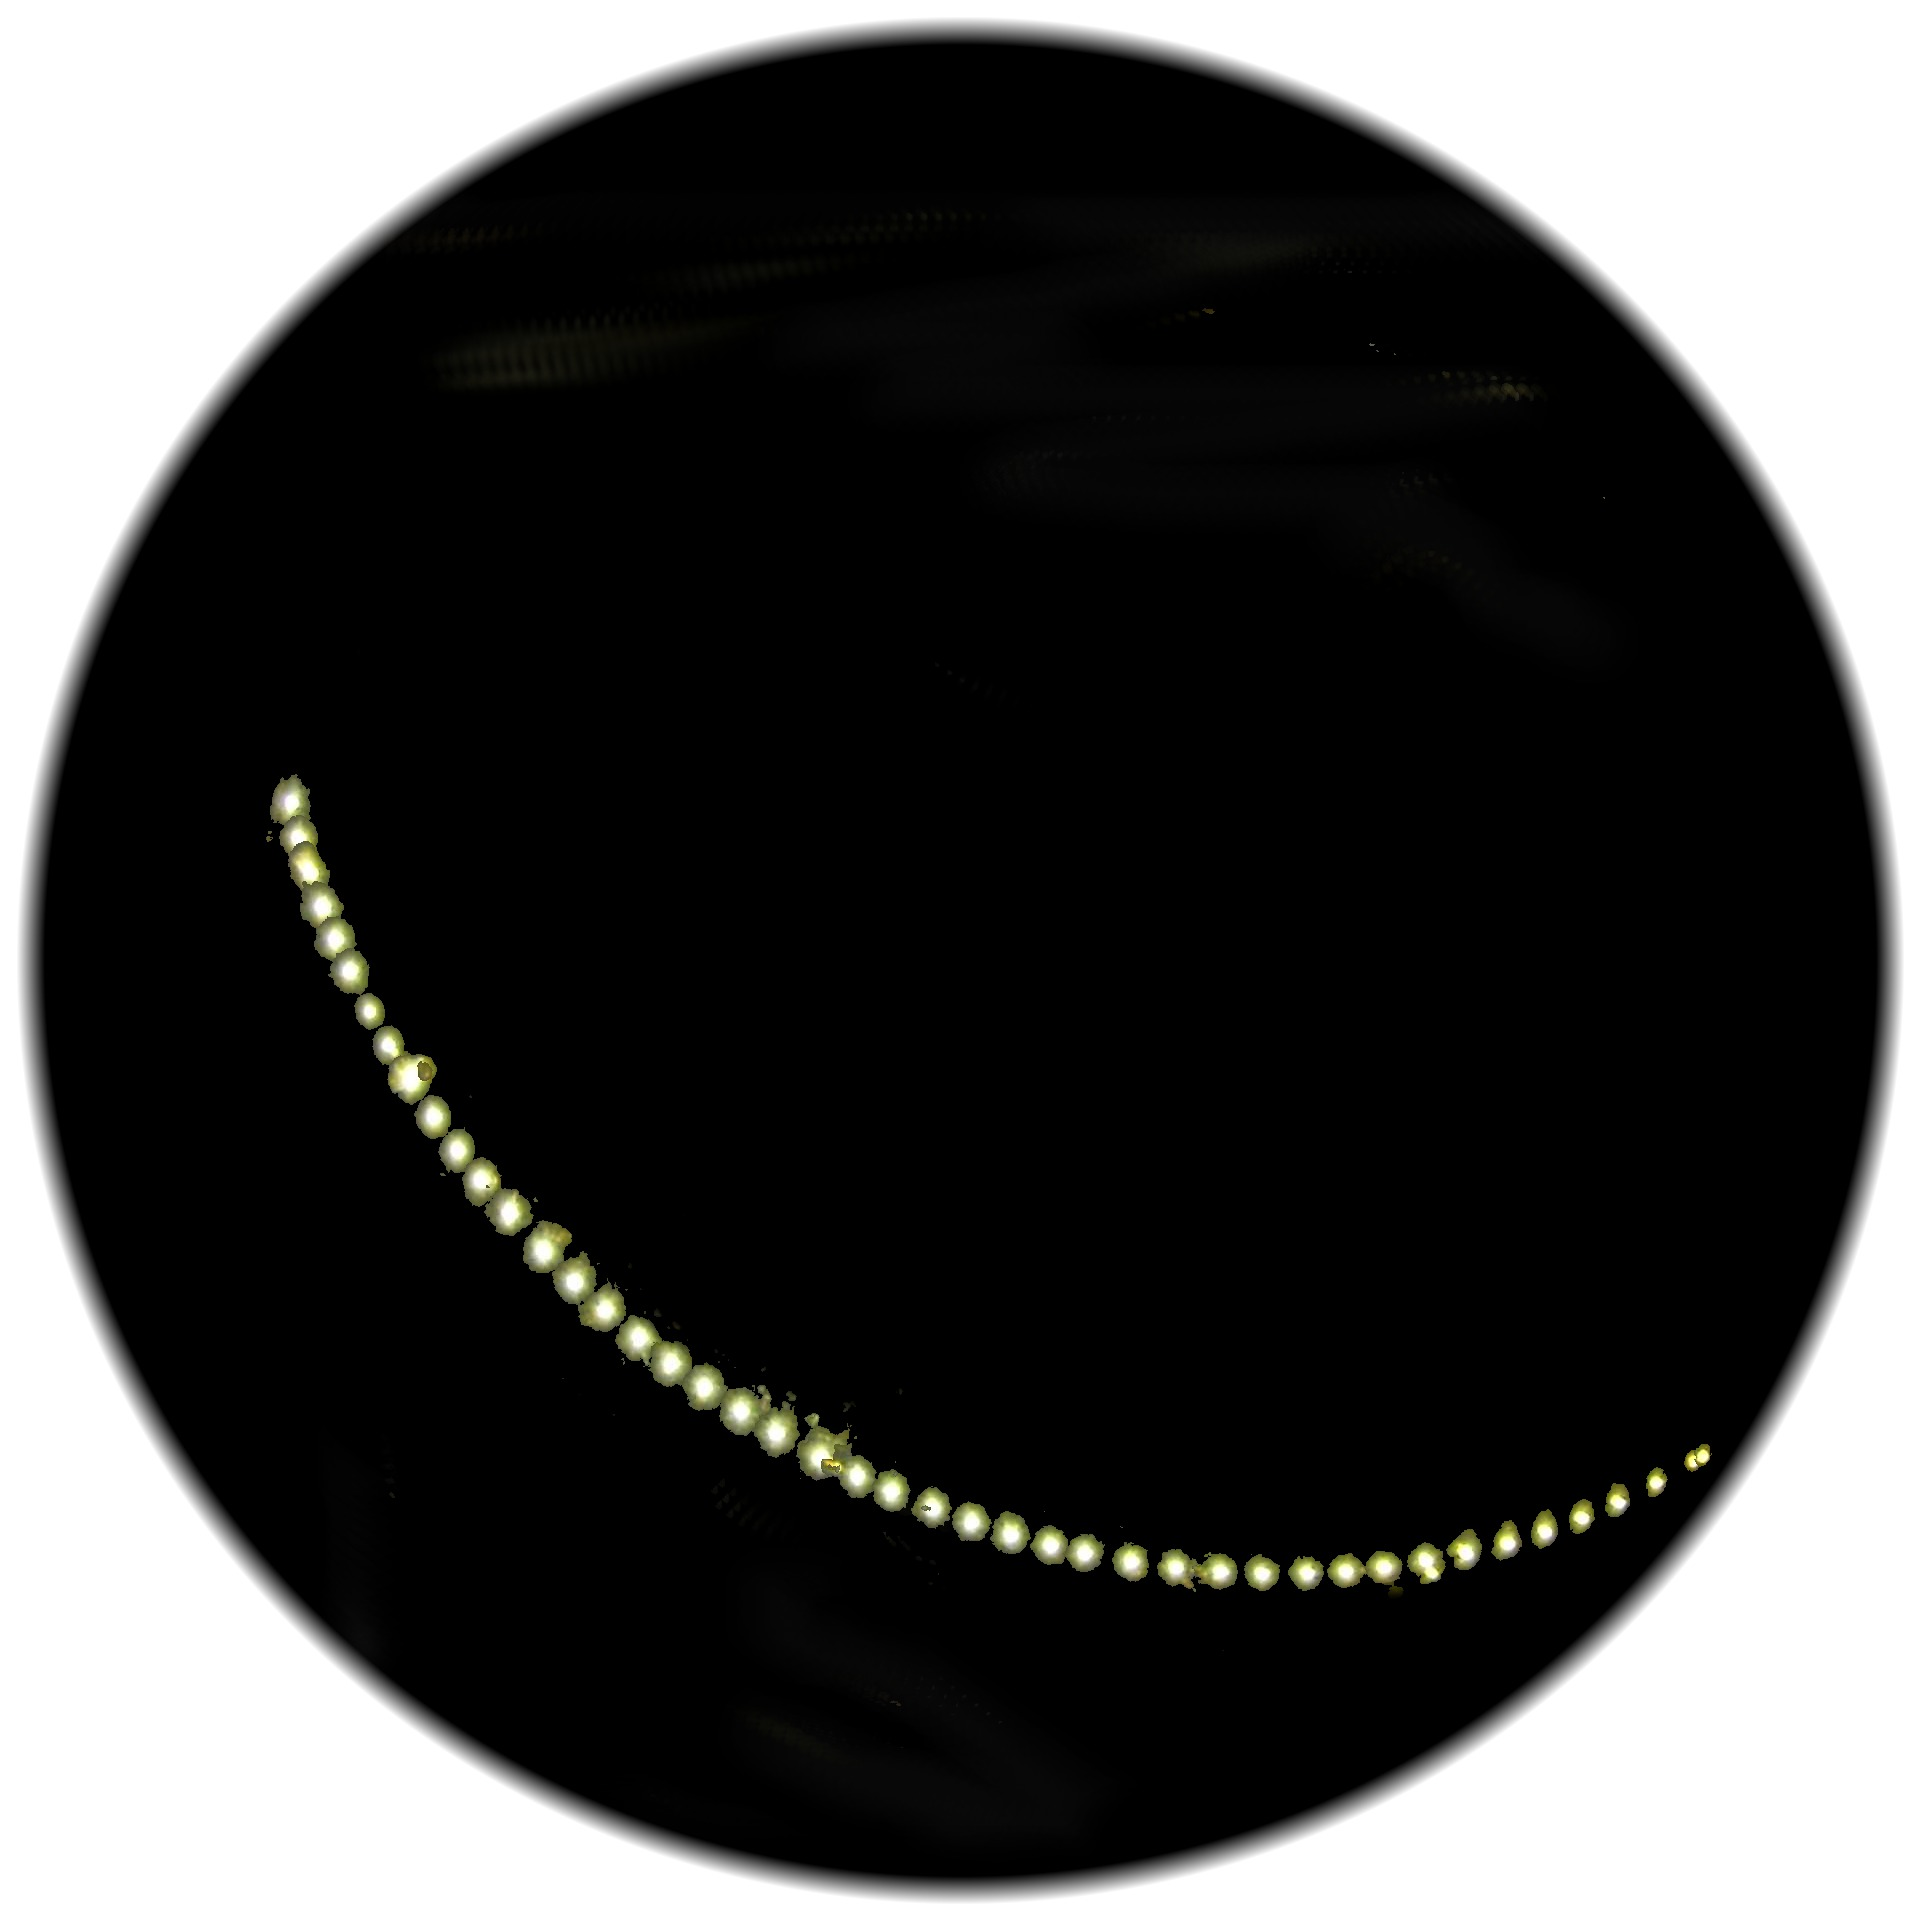
\includegraphics[width=0.22\textwidth]{media/cam3_straight_gold.jpg} &
        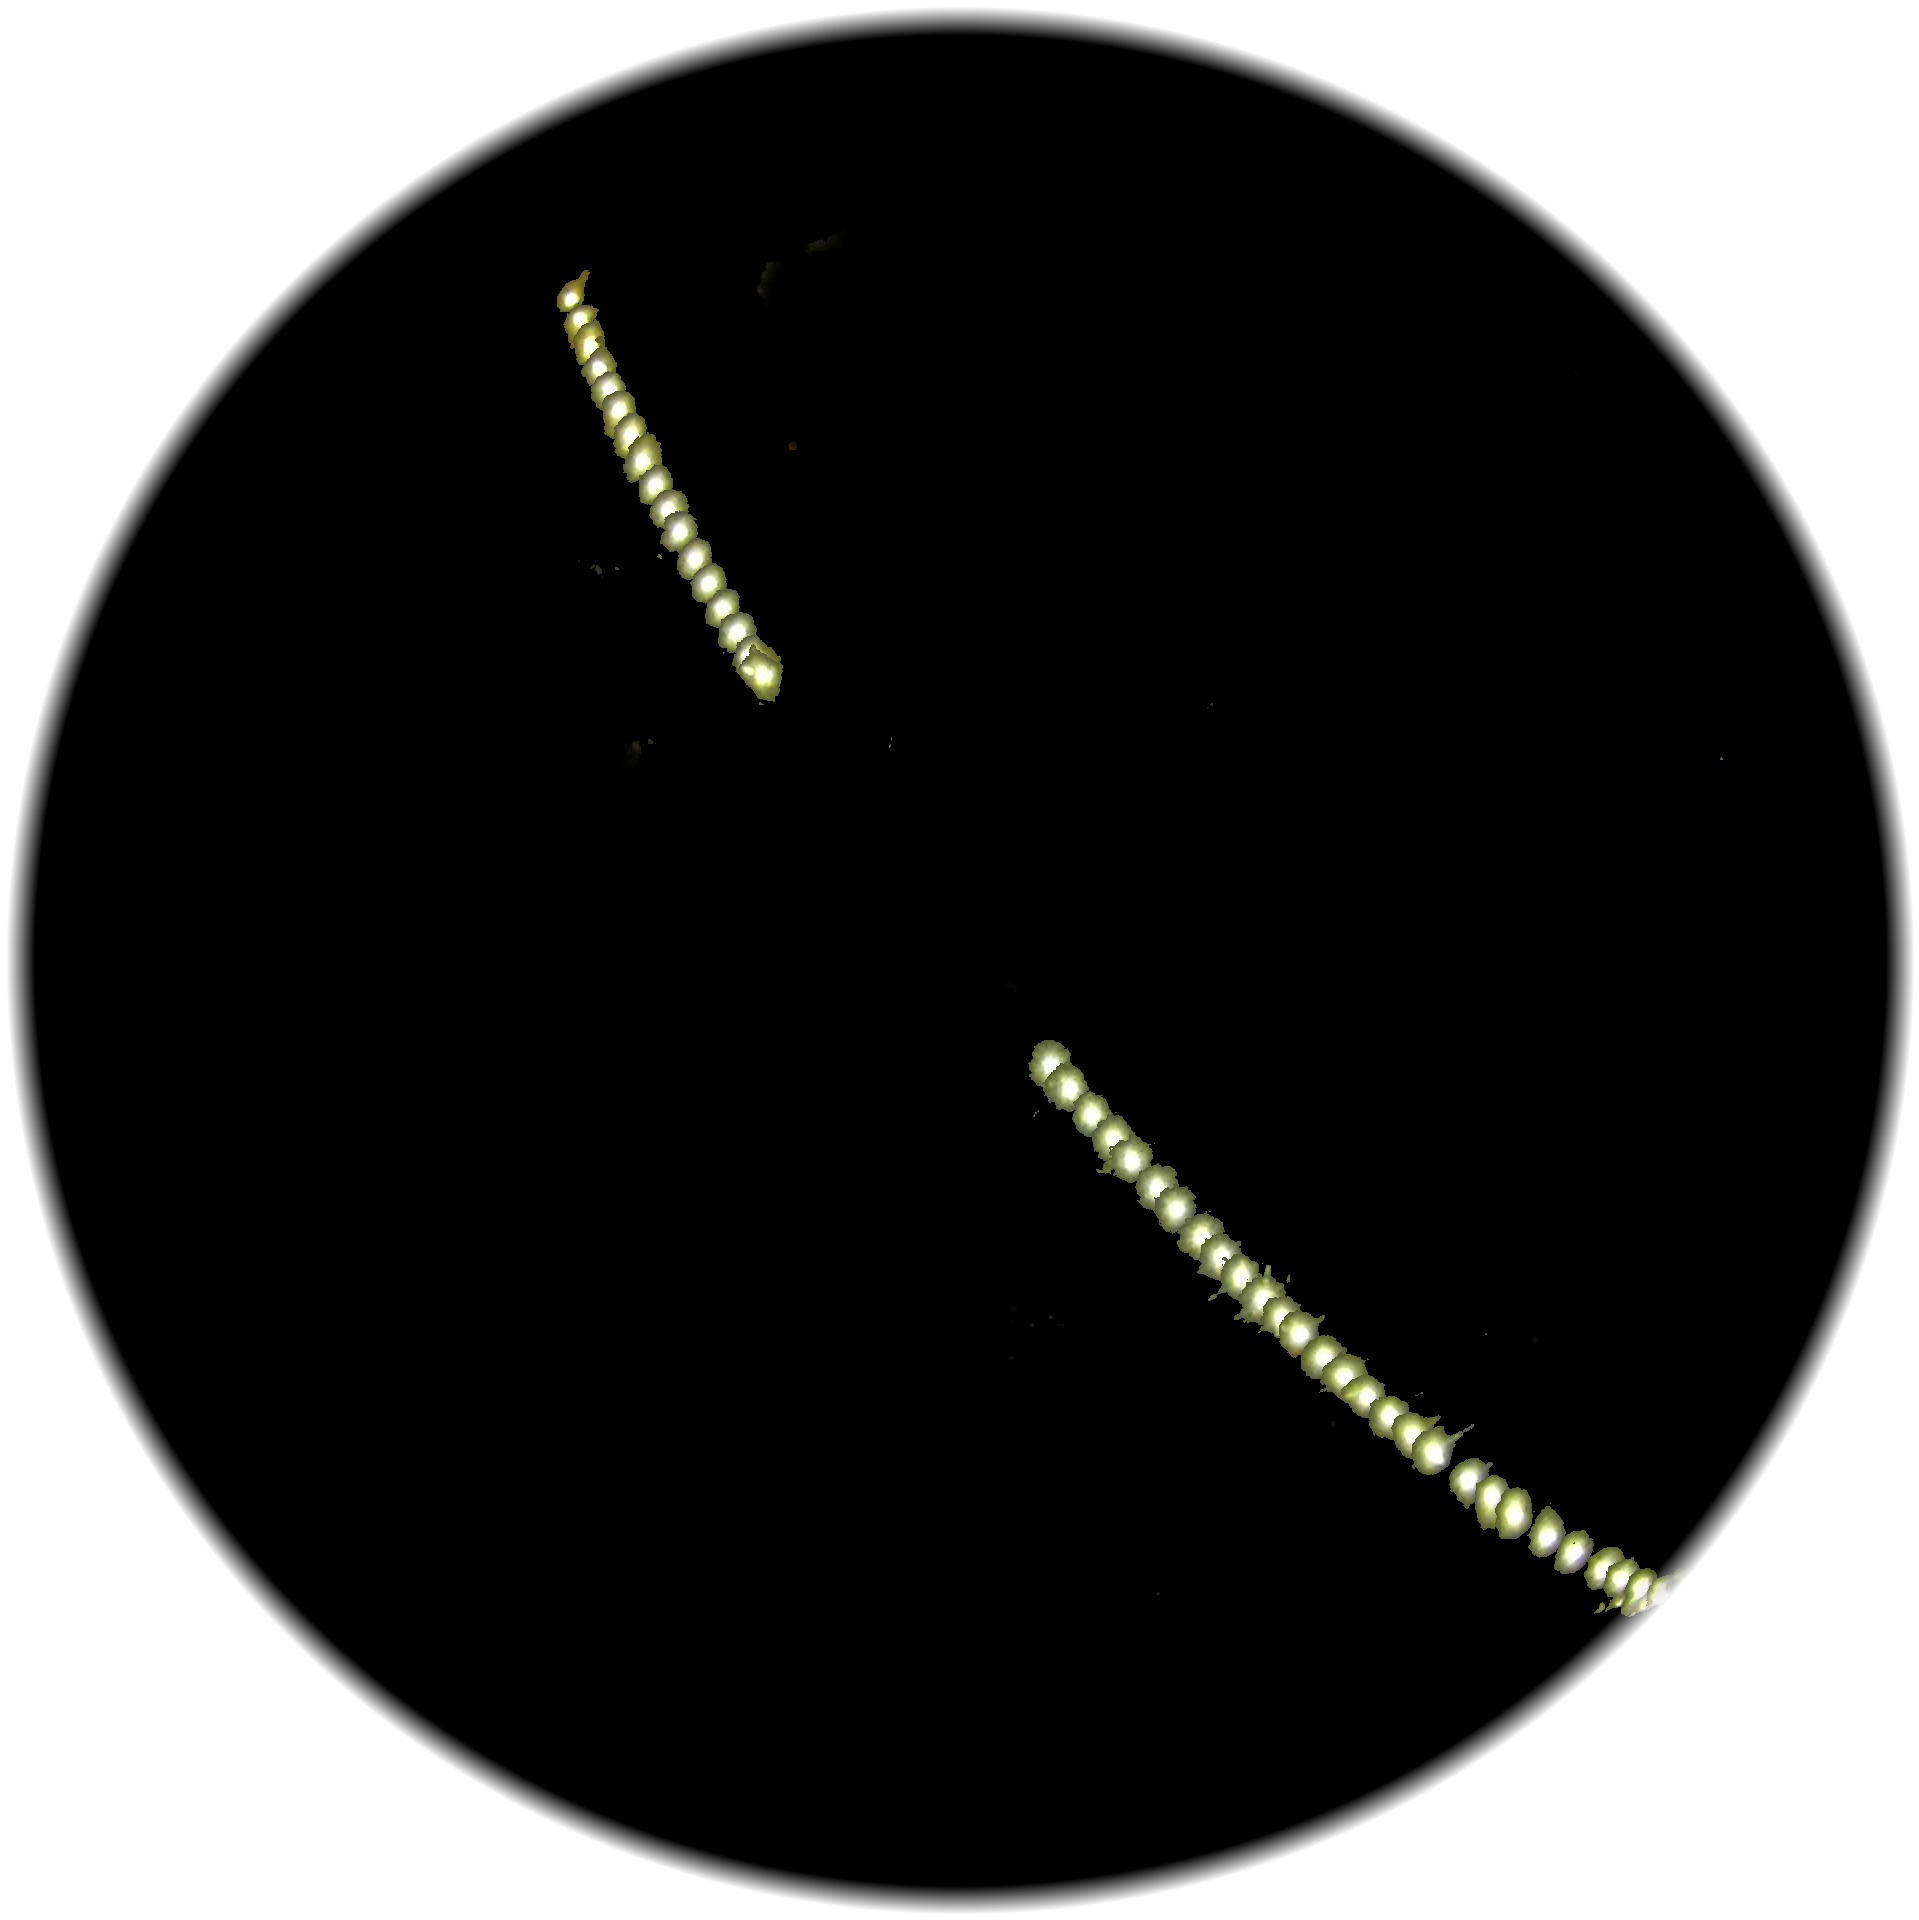
\includegraphics[width=0.22\textwidth]{media/cam3_proj_gold.jpg} \\
        (a) & (b) \\
    \end{tabular}
    }
    
\ffigbox{
    \caption[Projektion von Bildkoordinaten zu realen Koordinaten]{Projektion
    von Bildkoordinaten zu realen Koordinaten: (1) Sonne auf dem Bild (2)
    Elevation wird aus Radialprojektion angenährt (3)\,-\,(5) Drehung im Raum
    durch Euler-Winkel.  Die Punkte\ (2)\,-\,(5) befinden sich auf der
    Einheitsphäre.}
    \label{FIGProjektion}
}{
    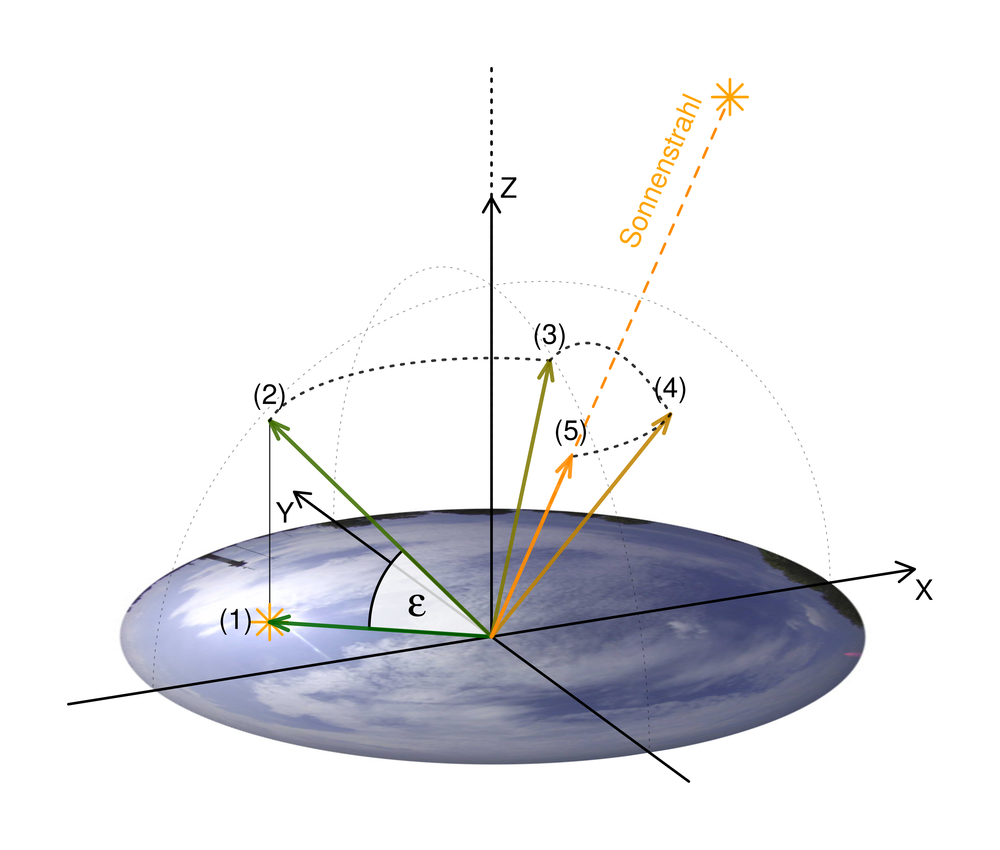
\includegraphics[width=0.49\textwidth]{media/calibration-chart.png}
}
\end{floatrow}
\end{center}
\end{figure}

\begin{figure}[!h]
\begin{center}
\vspace{-0.7cm}
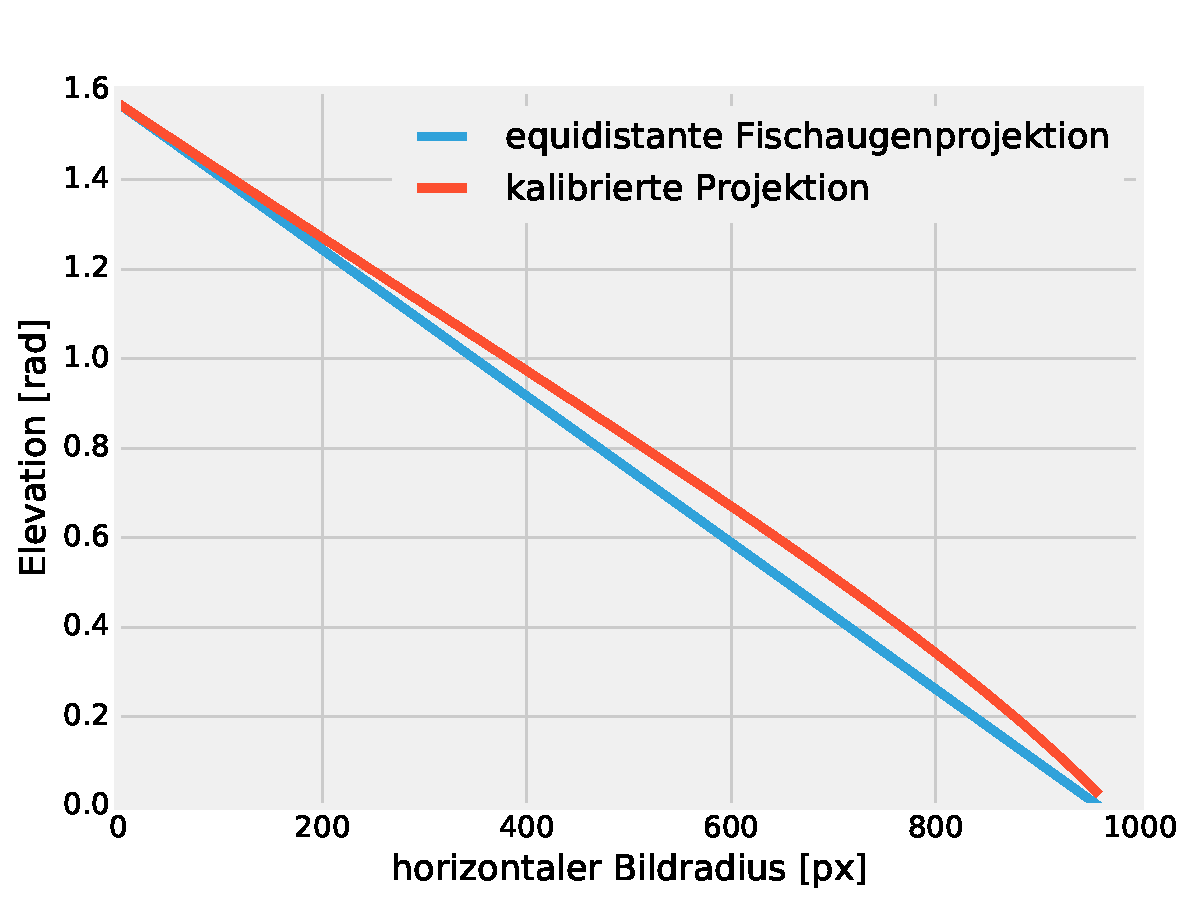
\includegraphics[width=0.5\textwidth]{media/projection-calibration.pdf}
\vspace{-0.7cm}
\caption[Kalibrierte Projektionsfunktion]{Kalibriertes Projektionspolynom im
Vergleich zur equidistanten Fischaugenprojektion}
\label{FIGProjektioncalib}
\end{center}
\end{figure}

%\newpage

%%%%%%%%%%%%%%%%%%%%%%%
%%% Wolkenerkennung %%%
%%%%%%%%%%%%%%%%%%%%%%%
\section{Wolkenerkennung}
\label{SECWolkenErkennung}
Die Wolkenerkennung ist der nächste Teil des hier verwendeten Ansatzes zur
Bestimmung der Wolkenbasishöhe. Sie gliedert sich in die folgende aufeinander
aufbauenden Schritte: Zunächst erfolgt für jeden Bildpixel die Kategorisierung,
ob es sich um einen Wolkenpixel handelt oder nicht.  Dann werden die
Wolkenpixel zu zusammenhängenden Wolken gruppiert. Schließlich werden zwei
zeitgleiche Bilder der unterschiedlichen Wolkenkameras zusammengeführt, um
passende Wolkenpaare zu finden. 

\subsection{Wolkensegmentierung} 
Der erste Schritt der Wolkenerkennung ist das Finden von Wolkenpixeln auf den
Bildern, im weiteren Verlauf Wolkensegementierung genannt. Die
Wolkensegmentierung soll dazu führen, ein möglichst fehlerfreies
Wolke/keine-Wolke Bild zu erhalten, also die Wolken aus dem Bild
herauszuschneiden.\absatz Die hier verwendeten Algorithmen basieren darauf, dass
die Farben der Bildpixel einer bimodalen Verteilung folgen, also ein Schwellwert
für die Segmentierung berechnet werden kann.  Die Wolkensegmentierung ist mit
den unbearbeiteteden RGB-Kanälen schwierig \citep{dev_14_color}, sodass
vorbereitende Schritte nötig sind, um Wolken aus einem Wolkenkamerabild zu
segmentieren.\absatz Im ersten vorbereitenden Schritt werden die Bilder lokal
zentriert. Beim lokalen Zentrieren wird die mittlere Helligkeit in einem Bereich
um diesen Pixel herum abgezogen. Dadurch wird die Helligkeit der Kamera
zentriert und der Einfluss der Sonne auf die Bildkanäle verringert. Im zweiten
vorbereitenden Schritt werden die drei Farbkanäle zu einem einzelnen
$\frac{Blau-Rot}{Blau+Rot}$-Kanal kombiniert. Das Blau-Rot Verhältnis ist
normalisiert und hat damit einen definierten Wertebereich zwischen -1 und 1. Bei
einem blauen Pixel liegt der Wert bei Eins, während bei einem weißen Pixel der
Wert bei Null ist. Durch das Blau-Rot Verhältnis ist es einfacher Wolken zu
finden.\absatz In unserem Ansatz wird das Wolkenkamerabild durch einen
Schwellwert im Blau-Rot Verhältnis segmentiert. Unterhalb dieses Schwellwertes
wird der Pixel als Wolke kategorisiert. Der Schwellwert besteht zu gleichen
Teilen aus einem vordefinierten und einem bildspezifischen Schwellwert.  Der
vordefinierte Schwellwert wurde durch den sogenannten K-Means Algorithmus
\citep{james_13_introduction} an vier manuell ausgewählten Testbildern
berechnet. Die vier Testbilder sind so ausgewählt, dass ein möglichst großes
Spektrum an Bewölkungsgraden und -arten abgedeckt ist. Der K-Means Algorithmus
berechnet die Mittelpunkte der beiden Kategorien – Wolke und nicht Wolke. Der
Schwellwert entspricht dem Mittelwert dieser beiden Mittelpunkte. Für den
bildspezifischen Schwellwert wird der sogenannte Otsu-Algorithmus benutzt
\citep{otsu_75_threshold}. Durch die Kombination des vordefininerten und des
bildspezifischen Schwellwertes wird sichergestellt, dass einerseits der
Schwellwert für verschiedenste Wolkentypen verwendet werden kann und
andererseits der Schwellwert für jedes Bild angepasst wird, um auch
bildspezifische Verteilungsbesonderheiten abzudecken.\absatz Aus der
Wolkensegmentierung wird die Information Wolke oder keine Wolke Pixelweise
gewonnen. Im nächsten Schritt werden die Wolkenpixel gruppiert, sodass
zusammengehörige Wolkenpixel als Teil einer Wolke erkannt werden.\absatz Um die
Wolken zu gruppieren wird das RGB-Bild mit dem Slic-Algorithmus in sogenannte
Superpixel unterteilt. Der Slic-Algorithmus basiert auf dem K-Means Algorithmus
und sorgt dafür das benachbarte Pixel, die ähnliche Farbwerte haben, gruppiert
werden. Diese Superpixel werden mit den segmentierten Wolkenpixel
zusammengeführt. Dafür werden Wolkenpixel die die dem gleichen Superpixel
entsprechen gruppiert. Durch den Superpixelansatz werden die Wolken in kleinere
Wolkenteile gruppiert.  Dadurch sollen im Datensatz richtig erkannte
Wolkenbasishöhen überwiegen, sodass Rauschen herausgefiltert werden kann.
\absatz Wenn die Wolken gruppiert sind, ist die Verarbeitung von einzelnen
Bildern beendet und die Wolken von den Stereo-Wolkenkamerabildern können
zusammengeführt werden.

%%%%%%%%%%%%%%%%%%%%%%
%%% Wolkenmatching %%%
%%%%%%%%%%%%%%%%%%%%%%
\subsection{Wolkenabgleich}
Für die Positionierung der Wolke muss erkannt werden, welche Wolkenteile auf
beiden Bildern wo zusammengehören. Dafür werden aus beiden Wolkenkamerabildern
die guppierten Wolkenteile einzeln rechteckig ausgeschnitten.\absatz Im nächsten
Schritt werden die ausgeschnittenen Wolkenteile aus beiden Kameras miteinander
verglichen. Der Vergleich zwischen zwei Wolkenteilen wird durch Korrelationen
gebildet. Hierfür werden die Wolkenteile gegeneinander verschoben und für jede
Verschiebung die normierte Grauwertkorrelation der überlappenden Bildteile
berechnet. Damit bei der Korrelation Helligkeits- und Kontrasteffekt der
Wolkenkamera keine Rolle spielen, werden die ausgeschnittenen Wolkenteile vor
der Korrelationsbildung standarisiert, sodass der Mittelwert des Grauwertes $0$
entspricht und die Standardabweichung $1$ ist. Es wird angenommen, dass
zusammengehörige Wolkenteile die höchste Korrelation zueinander haben und einen
bestimmten Korrelationsschwellwert ($0,95$) überschreiten. Desweiteren gibt es
die Annahme, dass die Wolkenteile um den Punkt der höchsten Korrelation
gegeneinander verschoben sind.\absatz Nachdem die Zusammengehörigkeit von zwei
Wolkenteilen erkannt worden ist, kann die Höhe aus den dazugehörigen Winkeln
berechnet werden.
%\newpage


%%%%%%%%%%%%%%%%%%%%%%%
%%% Höhenbestimmung %%%
%%%%%%%%%%%%%%%%%%%%%%%
\section{Berechnung der Wolkenbasishöhe}
\label{SECHoehenbestimmung}
Wie in Abschnitt \ref{SECCalib} beschrieben hat jedes Wolkenkamerabild
zusätzlich zu den drei Farbkanälen eine Azimuth- und Elevationsmatrix, die für
jeden Pixel definiert ist. Diese Winkelinformation werden benutzt, um die
Wolkenbasishöhe aus den zusammengehörigen Wolkenteilen zu berechnen. Die
Wolkenbasishöhe wird für jeden überlappenden Pixel mit Hilfe des
Doppelanschnitts berechnet. Der Algorithmus des Doppelanschnitts ist im
Unterkapitel \ref{SECDoppel} beschrieben. Es kann davon ausgegangen werden, dass
jeder der bisherigen Schritte Fehler produziert, die sich aufsummieren und so
die berechnete Wolkenbasishöhe beeinflussen. Deshalb werden die Daten des
Doppelanschnitt nachbearbeitet. Dieser Filterungsprozess wird in Unterkapitel
\ref{SECHeightPost} aufgezeigt.

\subsection{Doppelanschnitt}
\label{SECDoppel}
Aus den Kamerabildern erhalten wir pro Pixelpaar 4 Winkelinformationen. Um die
Position im Raum zu bestimmen, werden jedoch nur drei Informationen benötigt.
Somit gibt es eine Information zu viel. Dadurch handelt es sich um ein
überbestimmtes Gleichungssystem. Mit Hilfe des Doppelanschnitts wird versucht,
eine bestmögliche Position aus diesem Gleichungssystem zu berechnen
\citep{lange_16_praktikum}.
\absatz
Aus den beiden Winkeln, die sich für einen Pixel auf der Wolkenkamera ergeben,
lässt sich ein Vektor im 3D-Raum formen (im folgenden Sichtlinie genannt), der
jedoch eine unbekannte Länge hat. Es ist bekannt, welche Pixel auf den beiden
Kameras zusammengehören und so können Paare von Sichtlinien gebildet werden.
Zwei Sichtlinien schneiden sich allerdings durch das überbestimmte
Gleichungssystem im 3D-Raum nie. Um dieses Problem zu lösen, wird im
Doppelanschnitt angenommen, dass die Position im 3D-Raum dem Mittelpunkt der
kürzesten Verbindungsgerade zwischen den beiden Sichtlinien entspricht
(Abb.~\ref{FIGDoppel3d}).

\begin{figure}[h]
	\begin{center}
		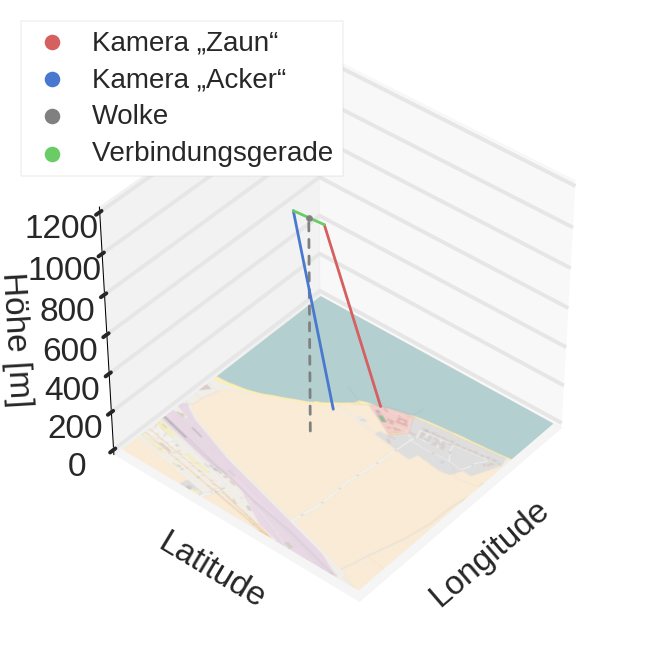
\includegraphics[width=0.6\textwidth]{media/3d.png}
		\caption[Darstellung des Doppelanschnitts]{Darstellung eines Wolkenpunktes im 3D-Raum mit den beiden Sichtlinien der Kameras und der kürzesten Verbindungsgeraden \footnotemark}
		\label{FIGDoppel3d}
	\end{center}
\end{figure}

\subsection{Nachbearbeitung der Wolkenbasishöhen}
\label{SECHeightPost}

Die Wolkenbasishöhen aus dem Doppelanschnitt können für jedes Wolkenteilpaar
gebildet werden. Diese Daten können als zusätzliche Rohdaten angesehen werden,
die aus den Kamerainformationen gewonnen werden. Durch mehrere Gründe sind die
Rohdaten fehlerbehaftet. Deshalb wird im folgenden die Nachbereitung der
Rohdaten beschrieben, damit die berechnete Wolkenbasishöhen mit den
Ceilometer-Wolkenbasishöhen vergleichbar sind.\footnotetext{Map data copyrighted
OpenStreetMap contributors and available from \url{openstreetmap.org}}\absatz Es
wird davon ausgegangen, dass Wolkenbasishöhen nur in einem bestimmten
Höhenbereich Sinn ergeben, von daher werden alle negativen Wolkenhöhen und
Wolkenhöhen über $10.000\,\mathrm{m}$ aus den Datensatz entfernt.\absatz Durch
Verschmutzung der Kamera und eine nicht perfekte Wolkenerkennung können
Wolkenfragmente entstehen, die keine Wolke darstellen.  Solange diese in einem
realistischen Höhenbereich sind, können diese durch den vorherigen Schritt nicht
aus dem Datensatz herausgenommen werden. Da aber davon ausgegangen werden kann,
dass die richtig erkannten Wolkenteile überwiegen, kann der Median für einen
Zeitraum gebildet werden. Der Median hat den Vorteil, dass Ausreißer, z.B.
falsch erkannte Wolkenfragmente, keinen so großen Einfluss auf den Mittelwert
haben, wie bei dem Erwartungswert.\absatz Die Kameras haben nur eine begrenzte
räumliche Auflösung und zusätzlich ist der Wol\-ken\-er\-ken\-nungs\-an\-satz
ein statistischer Ansatz, deshalb kann es innerhalb der Zeitreihe größere
Schwankungen geben. Um diese Schwankungen zu filtern, wird ein gleitender Median
über einen Zeitraum von 15~Minuten gebildet. Durch die gleitende Medianbildung
entsteht eine glatte Zeitreihe. Dies ist der letzte Schritt in der Filterung der
Wolkenkamera-Rohdaten.\absatz

%\newpage

%%%%%%%%%%%%%%%%%%%
%%% Validierung %%%
%%%%%%%%%%%%%%%%%%%
\section{Validierung}
\label{SECValidation}
Mit Hilfe der vorgestellten Methoden werden Wolkenbasishöhen berechnet. Um diese
auf ihre Richtigkeit zu überprüfen muss diese Evaluiert werden. Es kann
untersucht werden, wie sensitiv die Wolkenbasishöhe auf kleinere Störungen
reagiert (\ref{SECSens}). Ebenso kann auch validiert werden in wie weit die
Entfernung der beiden Kameras zueinander und die räumliche Auflösung dieser
ausreicht, um die Wolkenbasishöhe zu berechnen. Im letzten Evaluierungsschritt
werden die berechneten Wolkenbasishöhen für ein Fallbeispiel mit den
Wolkenbasishöhen aus dem Ceilometer verglichen.

\subsection{Sensitivität der Wolkenbasishöhe}
\label{SECSens}
Um die Sensitivität der Wolkenbasishöhe auf Störung zu untersuchen wird hier
exemplarisch die Sensitivität des Wolkenpunktes aus Abb.~\ref{FIGDoppel3d}
untersucht.\absatz Die berechnete Wolkenbasishöhe kann einerseits durch den
Wolkenabgleich einen Fehler enthalten und andererseits ist der Doppelanschnitt
nur eine Abschätzung der tatsächlichen Wolkenbasishöhe. Es wird angenommen, dass
die Störungen einem gaußischem Rauschen mit einer Standardabweichung von
$1^{\circ}$ entspricht ($\sim7$ Pixel) und durch die Fehler kein Bias entsteht.
Die Winkel der Wolkenkameras werden unabhängig voneinander 100.000 Mal gestört,
um eine Verteilung an möglichen Wolkenhöhen zu erhalten (Abb.
\ref{FIGSens}).\absatz Durch die Störungen entsteht eine schiefe Verteilung, die
wie wir annehmen einer rechtslastigen Gumbel-Verteilung folgt. Die Verteilung
hat ihren Modus bei einer geringeren Wolkenhöhe (zwischen $1000$ und
$1050\,\mathrm{m}$) als die aus den Daten berechnete Wolkenhöhe (Wahrheit
genannt, $~1085$ m Höhe). Der Median und der Mittelwert stimmen mit der Wahrheit
bis auf wenige Meter überein.\absatz Es zeigt sich, dass durch die Störungen
eine Schwankungsbreite von $\sim320\,\mathrm{m}$ in der Wolkenbasishöhe
entsteht. Die Schwankungen bleiben jedoch in einem Rahmen, der es erlaubt mit
unseren Methoden die Wolkenbasishöhe zu bestimmen.

\begin{figure}[t]
	\begin{center}
		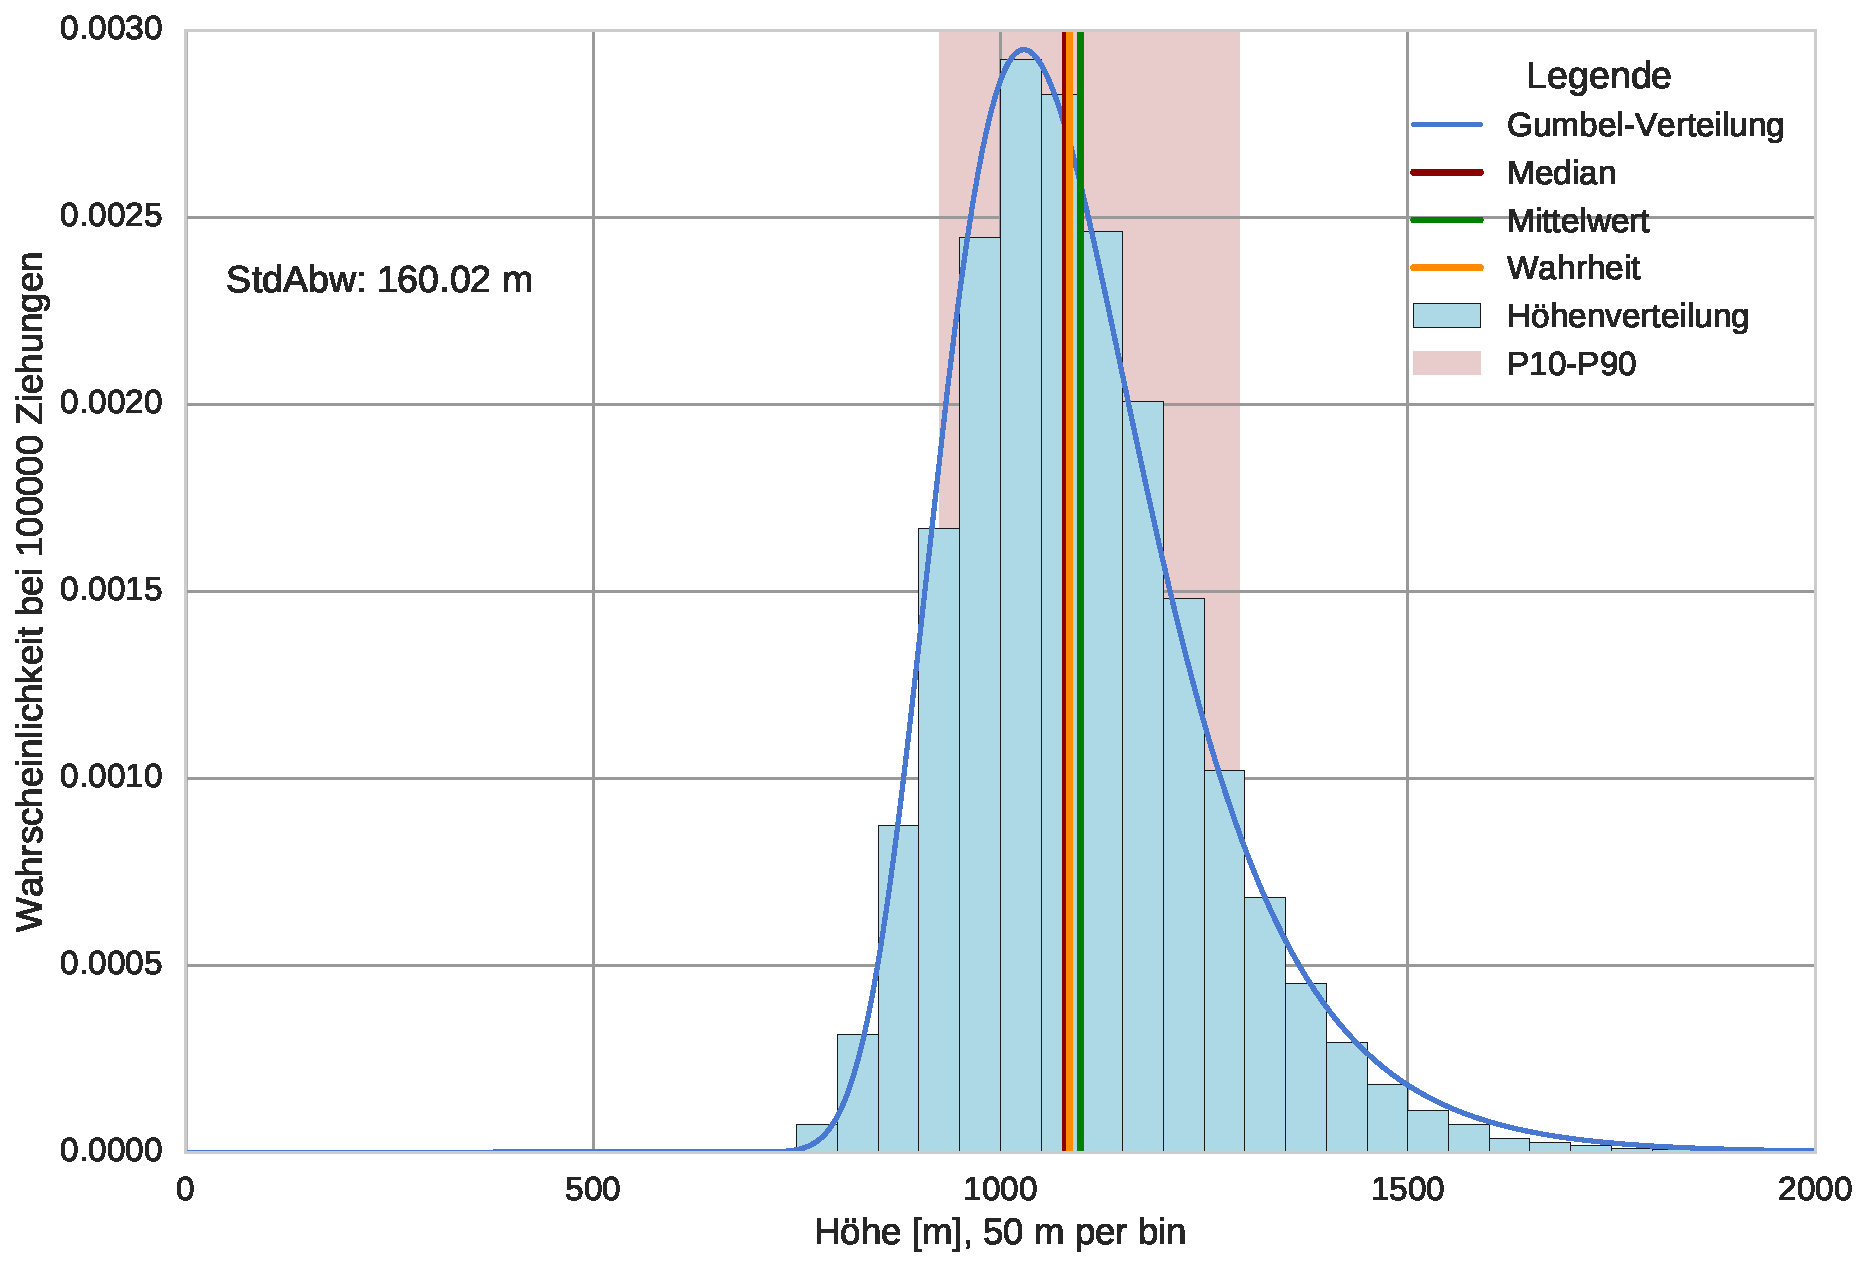
\includegraphics[width=0.75\textwidth]{media/sens_prob_height.pdf}
		\caption[Wolkenhöhenverteilung von gestörten Wolkenkamerawinkeln]{Darstellung einer Verteilung von Wolkenbasishöhen bei gestörten Wolkenkamerawinkeln. In Blau ist die berechnete Gumbel-Verteilung zu sehen. Der Median, der Mittelwert und die nicht gestörte Wolkenhöhe (Wahrheit) sind mit einem roten, grünen bzw. gelben Strich gekennzeichnet. Das 10\% bis 90\%-Perzentil wird im Hintergrund mit einer rötlichen Fläche gezeigt. Die Standardabweichung wurde mit der gezeigten Gumbel-Verteilung berechnet}
		\label{FIGSens}
	\end{center}
\end{figure}

\subsection{Vergleich zwischen Drachenhöhen aus Wolkenkameras und aus Theodoliten}
\label{SECDragon}
Um zu überprüfen, ob die Entfernung und räumliche Auflösung der beiden
Wolkenkameras ausreicht, werden die Daten von Theodolitenmessungen für ein
bestimmtes Sichtziel (Lastendrachen) mit den berechneten Höhen der beiden
Wolkenkameras verglichen.\absatz Die beiden Theodoliten werden neben die Kameras
gestellt, damit die beiden Messsysteme vergleichbare Ergebnisse liefern. Die
Theodoliten nehmen in fünfsekündigen Schritten die anvisierten Raumwinkel auf.
Aus den vier Raumwinkeln kann wie bei den Wolkenkameras mit Hilfe des
Doppelanschnitts die Position des Sichtziels berechnet werden.\absatz Das
Sichtziel ist in diesem Experiment ein Lastendrachen mit einer Spannweite
von\linebreak[4]$3~\text{m}~\cdot~1,80~\text{m}$. Der Drachen stieg bei den beiden
Aufstiegen bis auf um die $100\,\mathrm{m}$ Höhe.\absatz In diesem Experiment
wird die Drachenposition bei den beiden Wolkenkamerabildern manuell markiert, um
ausschlißen zu können, dass der Fehler durch Algorithmen entsteht. Die jeweilige
Drachenposition für zwei Winkelpaare wird mit dem Doppelanschnitt ohne
Nachbearbeitung berechnet.\absatz

\begin{figure}[h]
	\begin{center}
		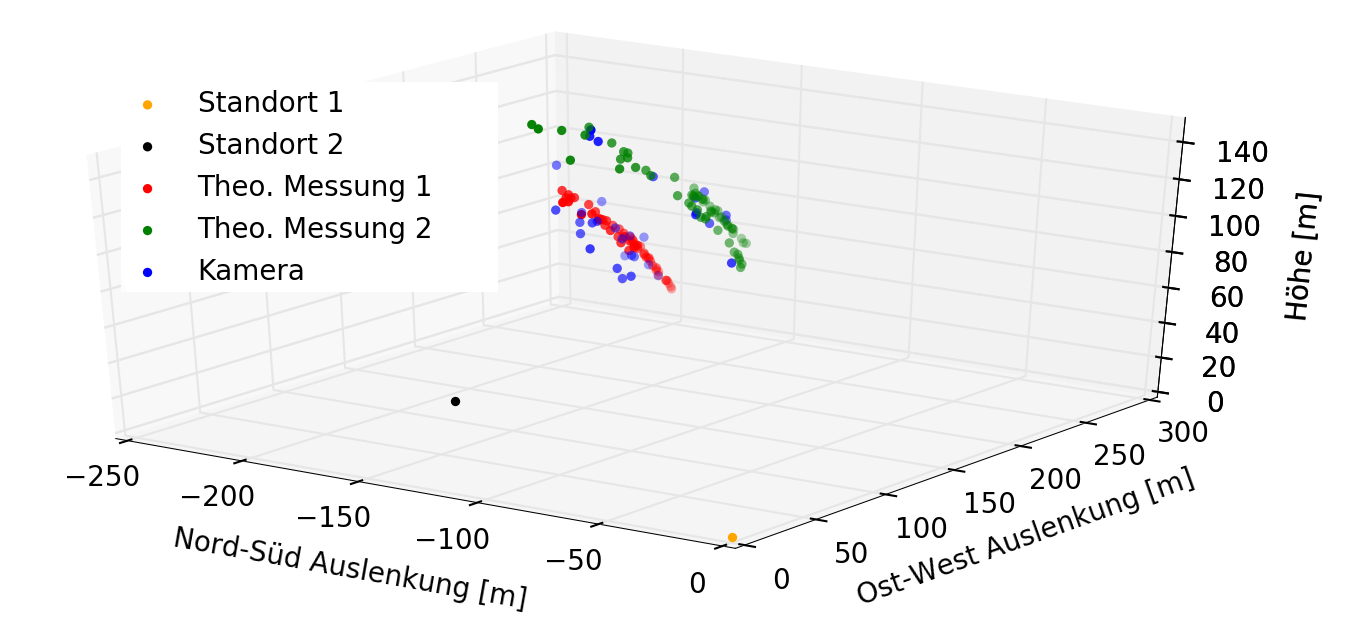
\includegraphics[width=1\textwidth]{media/dragon_theo.png}
		\caption[Drachenaufstieg]{Darstellung der beiden Drachenaufstiege berechnet mit Theodoliten und den Wolkenkameras.  Die Drachenhöhen, berechnet mit den Kameras, sind in Blau dargestellt, während die Drachenhöhen berechnet aus Theodolitdaten in Rot und Grün dargestellt sind}
		\label{FIGTheoDragon}
	\end{center}
\end{figure}

Wie in Abb.~\ref{FIGTheoDragon} zu sehen ist, stimmen die berechneten Positionen
der beiden Messsysteme bis auf wenige Meter überein. In den Daten ist eindeutig
zu sehen, dass die Wolkenkameras eine geringere zeitliche Auflösung als die
Theodoliten haben und so den zeitlichen Verlauf der beiden Drachenaufstiege
nicht so genau wiedergeben kann. Zwischen den beiden Drachenaufstiegen lag eine
Pause von ca. 10 Minuten, bei der die Position des Drachen geändert wurde. Es
ist ersichtlich, dass trotz der veränderten Drachenposition der Unterschied in
der Wolkenhöhe, berechnet mit den beiden Messsystemen, sich nicht geändert hat
und somit das Ergebnis aussagekräftig ist.\absatz Dadurch, dass die
Wolkenkameramessungen mit den Theodolitenmessungen bis auf wenige Meter
übereinstimmen, kann geschlussfolgert werden, dass Abstand und die räumliche
Auflösung der beiden Kameras ausreichen, um die Wolkenbasishöhe zu bestimmen.
Die Unterschiede zwischen den Messsystemen sind durch die räumliche und
zeitliche Auflösung dieser, sowie durch die manuelle Markierung der Drachen auf
den Kamerabildern zu erklären. Die Ergebnisse zeigen, dass Fehler bei der
Bestimmung der Wolkenbasishöhe vorallem durch die Wolkenerkennung und nicht
durch den Doppelanschnitt oder die räumliche Auflösung entstehen.

\subsection{Vergleich der Wolkenbasishöhen aus Wolkenkameras mit einem Ceilometer}
\label{SECCeilo}
Um die berechneten Wolkenbasishöhen der Wolkenkameras mit den aus dem Ceilometer
zu vergleichen, wird im folgenden ein Fallbeispiel gezeigt, wo anfägnlich
Cumulus-Bewölkung dominiert hat, während es gegen Ende einen Warmluftaufzug mit
den dazugehörigen Cirren und stratiformer Bewölkung gab.\absatz Die
Wolkenbasishöhen sind mit den vorherig beschriebenen Methoden aus den beiden
Wolkenkameras bestimmt worden. Als Referenzdaten werden die untersten erkannten
Ceilometerhöhen im gleichen Zeitraum benutzt.\absatz

\begin{figure}[h]
	\begin{center}
		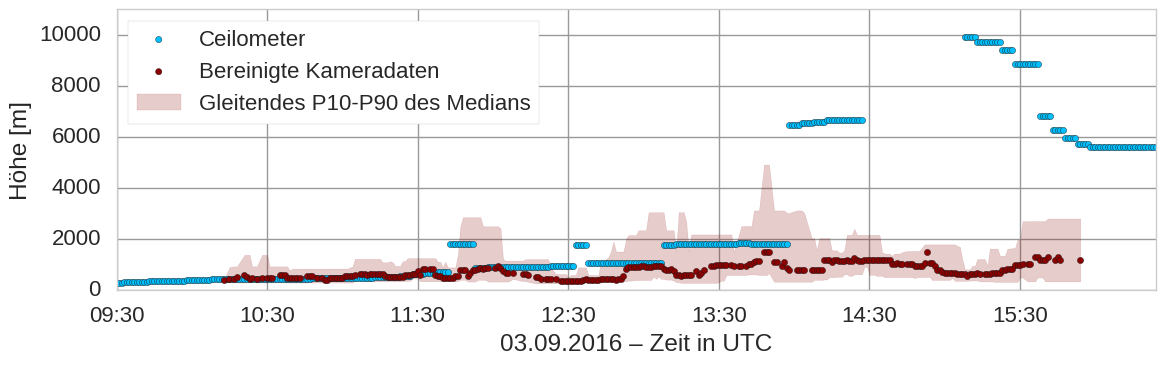
\includegraphics[width=1\textwidth]{media/ceilo_cam_new.png}
		\caption[Zeitreihenvergleich Wolkenkameras mit Ceilometer]{Darstellung eines Wolkenpunktes im 3D-Raum mit den beiden Sichtlinien der Kameras und der kürzesten Verbindungsgeraden}
		\label{FIGCeilo}
	\end{center}
\end{figure}

In Abb.~\ref{FIGCeilo} zeigt sich, dass bis zum frühen Nachmittag (ca.
13:40~Uhr) die Wolkenbasishöhen der beiden Methoden übereinstimmen. Diese
Periode ist durch Cumulus-Bewölkung geprägt und kann somit durch niedrige Wolken
charakterisiert werden. Die Zeitreihe des gleitenden Median kann die
zwischenzeitlich erhöhte Wolkenhöhen nicht wiedergeben. Die erhöhten
Schwankungen im gleichen Zeitraum, dargestellt mit den gleitenden Perzentilen,
zeigt jedoch, dass die Wolkenkamera auch Wolken in den Höhen erkannt hat. Daraus
kann geschlussfolgert werden, dass in den Perioden die falsch erkannten
Wolkenteile einen größeren Einfluss haben, als die richtig erkannten
Wolkenteile. Dies kann unterschiedliche Gründe haben. Die Kamera kann
verschmutzt gewesen sein, sodass die Sonne in der Kamera reflektiert worden ist
und diese Reflektionen als Wolke erkannt worden sind. Diese These wird dadurch
unterstützt, dass in Perioden, in denen das Ceilometer keine Wolken erkannt hat,
die Wolkenkamera Wolken in ähnlichen Höhen wie am Vormittag erkannt hat. Es kann
auch die angewendete Methodik zur Wolkenerkennung Fehler haben, sodass z.B.
beleuchteter Himmel auch als Wolke erkannt wird.\absatz Die Periode in der es
den Warmluftauzug gibt und die somit mit hohen Cirren bzw. stratiformer
Bewölkung beschrieben werden kann, ist in den Daten der Wolkenbasishöhen aus der
Wolkenkamera nicht ersichtlich. Dies bedeutet, dass diese Wolken durch die
Wolkenkamera nicht oder zu wenig erkannt worden sind. Dadurch lässt sich sagen,
dass in dem Fall der hohen Bewölkung mit sehr großer Wahrscheinlichkeit die
Wolkenerkennung nicht funktioniert hat und somit nur noch das Rauschen durch
falsch erkannte Wolkenteile zu erkennen ist. Die Schwankungen innerhalb der
Zeitreihe sind gegenüber der berechneten Wolkenbasishöhen am Vormittag größer
geworden. Deshalb kann auf Basis von diesen Erkenntnissen davon ausgegangen
werden, dass die berechneten Höhen bei der Cumulus-Bewölkung durch richtig
erkannte Wolken entstanden sind. Deshalb kann gesagt werden, dass die Methodik
bei tiefer, cumuliformer Bewölkung funktioniert, während sie bei hoher Cirrus,
bzw. stratiformer Bewölkung Probleme zeigt.  

%\clearpage


%%%%%%%%%%%%%
%%% Fazit %%%
%%%%%%%%%%%%%
\newpage
\section{Fazit}
Es wurde eine neue Methode zur Kalibration von Wolkenkameras entwickelt. Anhand
der Sonnenposition auf den Wolkenkamerabildern wurden die Bildkoordinaten sowie
die Projektion der Kamera kalibriert und ausgerichtet. Dadurch ist es nicht
mehr notwendig, Wolkenkameras exakt gerade aufzubauen und zu norden. Zusätzlich
ist es möglich, jegliche radiale Projektion zu korrigieren. Des Weiteren
wurde eine Methode gezeigt, um aus einem Stereo-Wolkenkamera-Aufbau die
Wolkenpositionen abzuschätzen. Mit statistischen Algorithmen wurden Wolkenteile
auf den Bildern erkannt. Mit dem klassischen Doppelanschnitt konnte aus
Wolkenpixelpaaren die Position dieser im 3D-Raum bestimmt werden. Es zeigte
sich, dass durch Ungenauigkeiten eine Schwankung von um die $100\,\mathrm{m}$
entstehen kann, diese jedoch gegenüber den Fehlern der Wolkenerkennung
vernachlässigbar sind. Es zeigt sich ebenso, dass diese Fehler in den
Algorithmen der Wolkenerkennung entstehen, da ein direkter Vergleich zwischen
Theodoliten und Wolkenkameramessungen - ohne Wolkenerkennung - vergleichbare
Ergebnisse liefert. Ein Vergleich mit dem Ceilometer hat gezeigt, dass die
Algorithmen bei tiefen Wolken funktionieren, während mittelhohe und hohe
Bewölkung Probleme bereiten.\absatz So muss als Fazit gezogen werden, dass noch
einiges an Arbeit hinein gesteckt werden muss, damit ein
Stereo-Wolkenkamera-Aufbau vergleichbare Ergebnisse zu einem Ceilometer liefern
kann. Diese Arbeit muss vorallem in die Algorithmen der Wolkenerkennung gesteckt
werden. Eine genauere Analyse von längeren Zeitreihen kann Erkentnisse liefern,
wie dies möglich ist.
%Als neuartige Methode könnten sich neuronale Netzwerke anbieten, die in anderen
%Bereichen der Bilderkennung neue State-of-the-Art Ergebnisse liefern.


%\newpage % Neue Seite

%%%%%%%%%%%%%%%%%%%%%%%%%%%%
%%% Literaturverzeichnis %%%
%%%%%%%%%%%%%%%%%%%%%%%%%%%%
\literaturverzeichnis{bibliography} % 

\end{document}
\grid
